% !TeX root = ../main.tex
\section{Evaluación Experimental y Resultados}
\label{sec:evaluacion}

En esta sección se analiza cuantitativamente el comportamiento del sistema a lo largo de las 30 rondas de entrenamiento federado, respondiendo a las preguntas de investigación formuladas: el sobrecoste temporal de la capa de auditoría, el comportamiento ante el escalado físico y de consenso, y el consumo de gas en la EVM.

\subsection{Convergencia del Modelo y Análisis de Pérdida}
La Figura~\ref{fig:convergencia} ilustra la evolución de la función de pérdida de entropía cruzada en el conjunto de validación durante las 30 iteraciones federadas.

\begin{figure}[H]
    \centering
    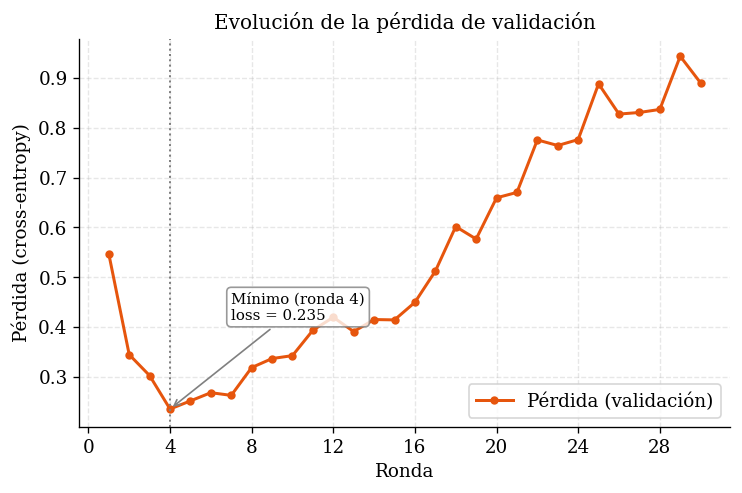
\includegraphics[width=\columnwidth]{figuras/convergencia_loss.png}
    \caption{Evolución de la pérdida de validación (\textit{cross-entropy}) a lo largo de las 30 rondas federadas.}
    \label{fig:convergencia}
\end{figure}

El modelo muestra un rápido aprendizaje inicial, alcanzando un mínimo de pérdida óptimo en la ronda 4 ($\mathcal{L} \approx 0{,}24$) con una precisión de clasificación que se estabiliza en el $97\%$. A partir de dicho punto, la pérdida experimenta un incremento gradual y sostenido hasta situarse en torno a $0{,}90$ hacia el final del ciclo. Este comportamiento representa un caso paradigmático de sobreajuste (\textit{overfitting}) provocado por el régimen de 90 épocas acumuladas (3 épocas locales $\times$ 30 rondas federadas) sobre un conjunto de entrenamiento acotado, donde la red incrementa excesivamente su confianza en predicciones.

El mínimo de pérdida en la ronda 4 sugiere que la incorporación de técnicas como la parada temprana (\textit{early stopping}) habría detenido el entrenamiento en ese instante, logrando una versión más ajustada del clasificador. Sin embargo, se mantuvieron de forma deliberada las 30 rondas predefinidas porque el objetivo central de esta investigación no es optimizar el modelo de IA ni perseguir su punto de máxima eficiencia, sino someter la infraestructura de aprendizaje federado a una carga constante para extraer métricas cuantitativas reproducibles (latencia por ronda, tiempo de confirmación y coste de gas). De este modo, la optimización fina del modelo se pospone como trabajo futuro.

Es fundamental enfatizar que \textbf{la curva de convergencia es estrictamente idéntica con o sin la presencia de Blockchain}. Dado que la capa de trazabilidad opera exclusivamente en la verificación e indexación criptográfica fuera de cadena y no interfiere en los tensores ni en los gradientes de FedAvg, la dinámica de entrenamiento se mantiene inalterada.

\subsection{Visión General del Rendimiento Temporal}
La Tabla~\ref{tab:tiempos_resumen} sintetiza el tiempo total requerido por ronda federada en las cinco configuraciones, reportando la mediana, media y desviación típica. Asimismo, la Figura~\ref{fig:tiempo_todas} refleja la serie temporal a lo largo de las 30 rondas.
\\

En la configuración distribuida E4 se registró una desviación típica notablemente superior (12,63 s) debida a un pico transitorio en la ronda 7 (121,3 s). Un análisis de rango intercuartílico confirmó que este valor anómalo obedeció a contención momentánea de memoria en el subsistema de virtualización WSL2. En consecuencia, se adopta la \textbf{mediana} como métrica central de referencia por su robustez frente a fluctuaciones esporádicas del entorno operativo.

\begin{table}[H]
\centering
\caption{Tiempo total de ejecución por ronda federada en cada configuración.}
\label{tab:tiempos_resumen}
\resizebox{\columnwidth}{!}{%
\begin{tabular}{cccccc}
\toprule
\textbf{Exp.} & \textbf{Máq.} & \textbf{Configuración} & \textbf{Mediana (s)} & \textbf{Media (s)} & \textbf{Desv. (s)} \\
\midrule
E1 & 1 & 4 val · con BC & 89,37 & 91,84 & 6,34 \\
E2 & 1 & Baseline sin BC & 84,15 & 82,18 & 6,95 \\
E3 & 2 & Baseline sin BC & 64,26 & 64,27 & 0,74 \\
E4 & 2 & 4 val · con BC & 71,29 & 77,05 & 12,63 \\
E5 & 2 & 7 val · con BC & 70,88 & 73,40 & 4,71 \\
\bottomrule
\end{tabular}%
}
\end{table}

\begin{figure}[H]
    \centering
    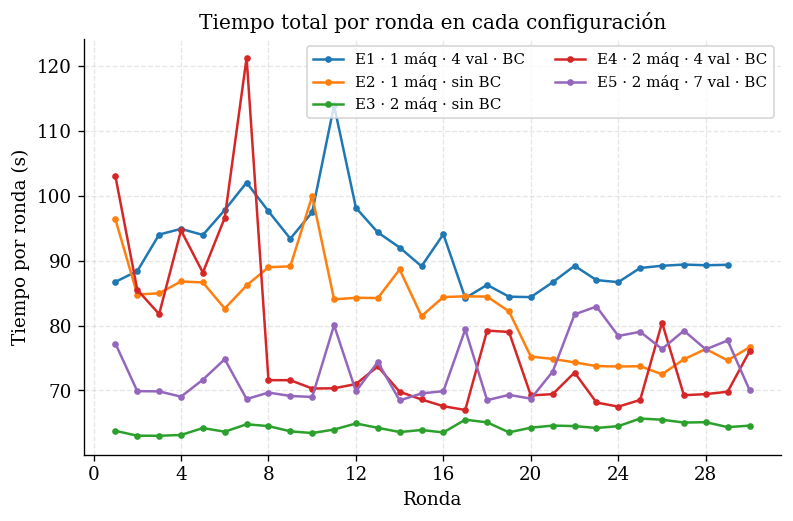
\includegraphics[width=\columnwidth]{figuras/tiempo_ronda_todas.png}
    \caption{Comparativa del tiempo total por ronda federada en las cinco configuraciones experimentales.}
    \label{fig:tiempo_todas}
\end{figure}

\subsection{Sobrecoste Temporal de la Capa Blockchain}
Para aislar el coste intrínseco impuesto por las llamadas a IPFS, las transacciones a la EVM y la sincronización con Besu, se comparan configuraciones que difieren únicamente en la inclusión de la Blockchain (Figura~\ref{fig:coste_bc}):
\begin{itemize}
    \item \textbf{Escenario Monomáquina (E1 vs. E2)}: El tiempo mediano pasa de 84,15 s a 89,37 s, lo que representa un sobrecoste de tan solo \textbf{5,22 s (+6,2\%)}.
    \item \textbf{Escenario Distribuido (E4 vs. E3)}: El tiempo mediano aumenta de 64,26 s a 71,29 s, suponiendo una sobrecarga de \textbf{7,03 s (+10,9\%)}.
\end{itemize}

\begin{figure}[H]
    \centering
    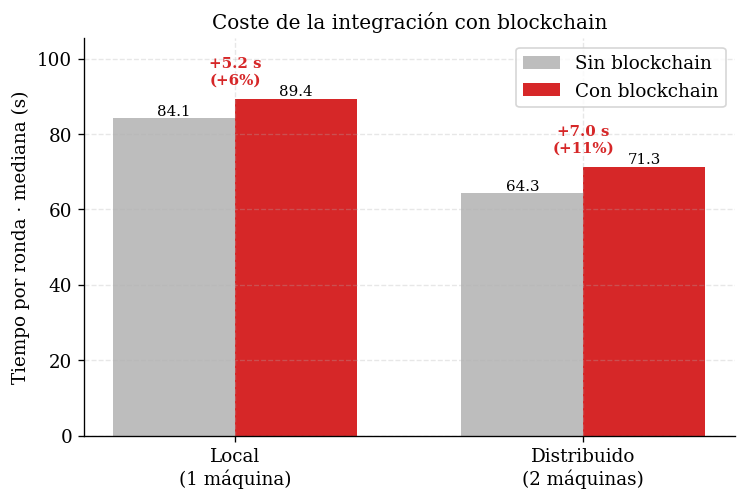
\includegraphics[width=\columnwidth]{figuras/coste_blockchain.png}
    \caption{Sobrecoste temporal inducido por la integración de la Blockchain en entornos local y distribuido.}
    \label{fig:coste_bc}
\end{figure}

Este incremento marginal ($\sim$5 a 7 segundos por ciclo) engloba la serialización con \texttt{pickle}, la publicación en IPFS, la firma ECDSA, la confirmación del bloque IBFT 2.0 y la verificación cruzada en cliente y servidor. Para sistemas que requieren auditoría legal o certificación de integridad, asumir un 10\% de penalización temporal constituye una penalización sumamente ventajosa.

\subsection{Efecto de la Distribución Física y Contención de Recursos}
La comparación entre una estación y dos estaciones revela un hallazgo crítico (Figura~\ref{fig:coste_dist}): distribuir los nodos en la red local \textbf{reduce drásticamente el tiempo de ronda}, tanto sin Blockchain (de 84,15 s a 64,26 s; una reducción de -23,6\%) como con Blockchain (de 89,37 s a 71,29 s; una reducción de -20,2\%).

\begin{figure}[H]
    \centering
    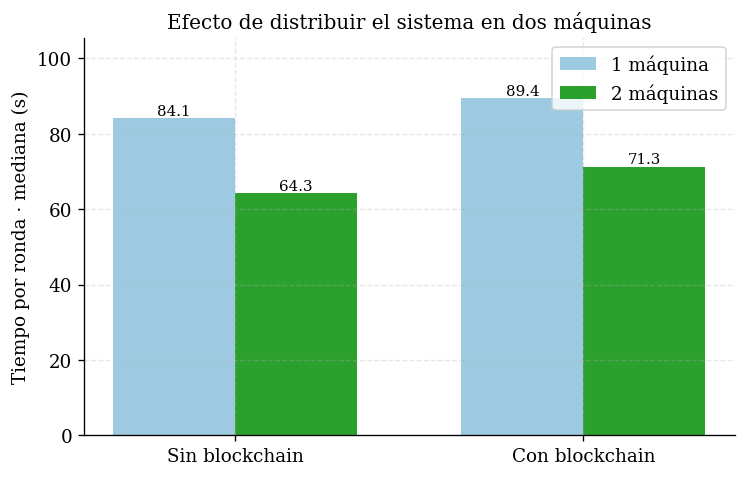
\includegraphics[width=\columnwidth]{figuras/coste_distribucion.png}
    \caption{Efecto de la distribución física de nodos sobre el tiempo de ciclo: mitigación de cuellos de botella de CPU/memoria.}
    \label{fig:coste_dist}
\end{figure}

La explicación reside en la eliminación de la contención de recursos. En la configuración local monomáquina, el daemon de Besu, los contenedores de validadores, IPFS y los procesos PyTorch compiten por los mismos 8 hilos y 7,6 GB de RAM. Al delegar la computación de los clientes a la Estación 2, la ganancia en capacidad de cómputo paralelo supera ampliamente la ligera latencia añadida por la transmisión de paquetes en la red inalámbrica.

\subsection{Impacto del Escalado de Validadores y Consenso IBFT 2.0}
Al comparar E4 (4 validadores) con E5 (7 validadores), el tiempo total de ronda se mantiene virtualmente indistinguible (71,29 s frente a 70,88 s). Esto confirma que el tiempo dominante en una ronda federada es la optimización neuronal local de los clientes, y no la latencia del bloque.

\begin{figure}[H]
    \centering
    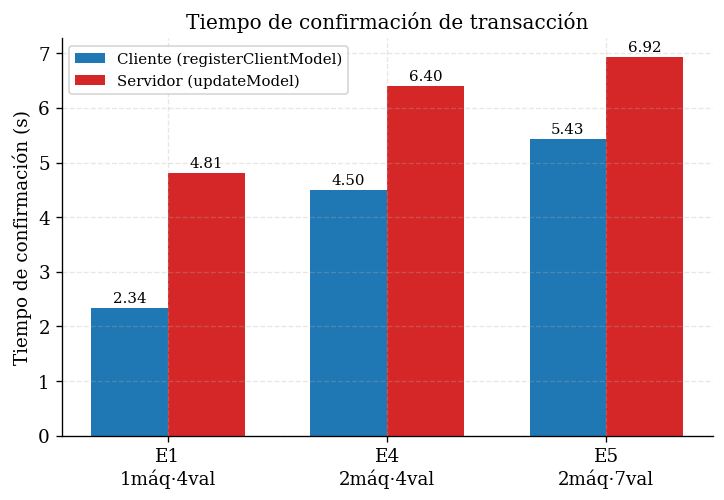
\includegraphics[width=\columnwidth]{figuras/tiempo_confirmacion.png}
    \caption{Tiempo medio de confirmación de transacción según topología y número de validadores en Hyperledger Besu.}
    \label{fig:tiempo_confirmacion}
\end{figure}

No obstante, al desagregar específicamente el \textbf{tiempo de confirmación de transacciones} (Figura~\ref{fig:tiempo_confirmacion}), el comportamiento del protocolo IBFT 2.0 se manifiesta nítidamente:
\begin{itemize}
    \item Para la transacción del cliente (\texttt{registerClientModel}), la latencia de confirmación crece de 4,50 s (con 4 validadores) a 5,43 s (con 7 validadores).
    \item Para la transacción del servidor (\texttt{updateModel}), el tiempo se eleva de 6,40 s a 6,92 s.
\end{itemize}
Este incremento lineal obedece a las fases de intercambio de mensajes (\textit{Prepare} y \textit{Commit}) del protocolo IBFT 2.0, que exige recabar firmas del quórum de supermayoría ($2f+1$). Sin embargo, este sobrecoste queda totalmente diluido en el tiempo total del entrenamiento, demostrando que elevar la tolerancia a fallos de $f=1$ a $f=2$ es viable sin penalizar el rendimiento macroscópico del sistema.

\subsection{Consumo y Previsibilidad del Gas en la EVM}
La Figura~\ref{fig:consumo_gas} ilustra el consumo de gas computacional de las operaciones registradas a lo largo de las rondas.

\begin{figure}[H]
    \centering
    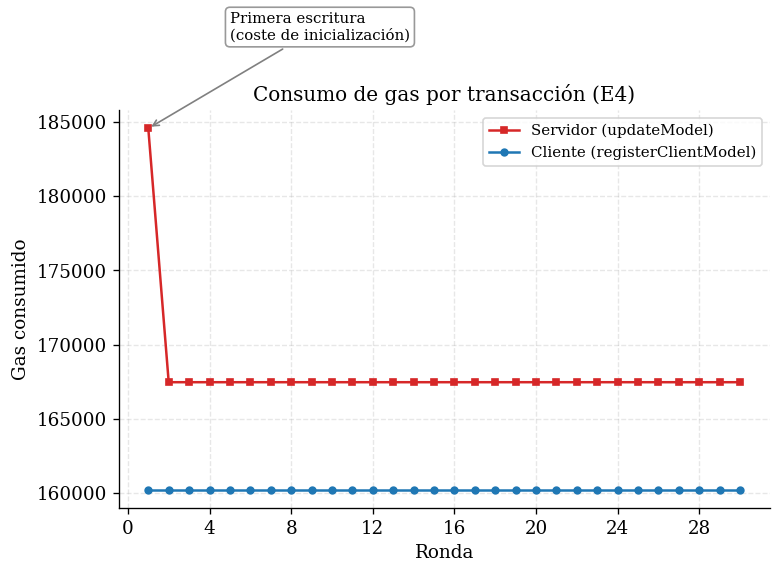
\includegraphics[width=\columnwidth]{figuras/consumo_gas.png}
    \caption{Consumo de gas en la Máquina Virtual de Ethereum por tipo de transacción a lo largo de las 30 rondas.}
    \label{fig:consumo_gas}
\end{figure}

El perfil de consumo resulta rigurosamente constante en todas las iteraciones subsiguientes:
\begin{itemize}
    \item \texttt{registerClientModel}: exactamente \textbf{160.200 unidades de gas}.
    \item \texttt{updateModel}: exactamente \textbf{167.460 unidades de gas}.
\end{itemize}
La única excepción observable corresponde a la ronda 0 del servidor, que demandó \textbf{184.560 unidades de gas}. Dicha discrepancia (+17.100 unidades) responde al coste intrínseco de la instrucción \texttt{SSTORE} de la EVM al escribir por primera vez en posiciones de memoria previamente vacías (\textit{cold write}) y modificar el valor del flag booleano \texttt{hasModel}.
\\

La invariabilidad del consumo valida formalmente el diseño desacoplado: al mantener almacenamiento de complejidad $\mathcal{O}(1)$ en el contrato (hashes y metadatos acotados), el coste en recursos computacionales es determinista e independiente del tamaño del modelo neuronal o del número de rondas ejecutadas.

